\documentclass[11pt]{article}
\usepackage{amsmath, amssymb, physics, mathtools, bm}
\usepackage{tikz, pgfplots}
\pgfplotsset{compat=1.18}
\usepackage[margin=2.3cm]{geometry}
\usepackage{siunitx, booktabs, hyperref}
\usepackage{braket}

\newcommand{\D}{\mathrm{D}}
\newcommand{\de}{\mathrm{d}}
\newcommand{\pd}[2]{\frac{\partial #1}{\partial #2}}
\newcommand{\pdd}[2]{\frac{\partial^{2} #1}{\partial #2^{2}}}
\newcommand{\Lap}{\nabla^{2}}

\title{B3 --- Quantum, Atomic and Molecular Physics --- Model Solutions, 2017}
\author{}
\date{}

\begin{document}
\maketitle

%====================================================================
\section*{Question 1 --- Spin-orbit interaction in hydrogenic atoms}

\textbf{Problem.} Derive the spin-orbit splitting for a hydrogenic atom and obtain
$\Delta E = Z^4\alpha^2 hcR_\infty / [n^3 l(l+1)]$. Apply numerically to $n=2,4$
of H, draw the level diagram for the Balmer-$\beta$ transition, and assess feasibility.

\subsection*{Derivation of $\Delta E$ ([9])}

Electron in rest frame sees motional magnetic field from nuclear Coulomb field.
Boost (non-relativistic): $\vb B' = -\vb v\times\vb E/c^2$.

Central field $\vb E = -(1/e)\,\vb\nabla V = (\vb r/r)(1/e)\,\de V/\de r$ with
$V(r)=-Ze^2/(4\pi\epsilon_0 r)$:
\[
\vb B' = -\frac{1}{c^2 e}\,\frac{1}{r}\frac{\de V}{\de r}\,(\vb v\times\vb r).
\]

Substitute $\vb L = m_e\,\vb r\times\vb v$, so $\vb v\times\vb r = -\vb L/m_e$:
\[
\vb B' = \frac{1}{m_e c^2 e}\,\frac{1}{r}\frac{\de V}{\de r}\,\vb L.
\]

Electron magnetic moment: $\vb\mu_s = -g_s\,\mu_B\,\vb S/\hbar$. Interaction
$H = -\vb\mu_s\cdot\vb B'$. Apply Thomas correction $g_s\to g_s-1\approx 1$:
\[
H_{\text{SO}} = \frac{1}{m_e c^2 e}\,\frac{1}{r}\frac{\de V}{\de r}\,\frac{\mu_B}{\hbar}\,\vb L\cdot\vb S.
\]

Insert $\mu_B = e\hbar/(2m_e)$ and $(1/r)\,\de V/\de r = Ze^2/(4\pi\epsilon_0)\cdot 1/r^3$:
\begin{equation}
H_{\text{SO}} = \frac{1}{2 m_e^2 c^2}\,\frac{Ze^2}{4\pi\epsilon_0}\,\frac{1}{r^3}\,\vb L\cdot\vb S.
\label{eq:HSO}
\end{equation}

First-order shift: $\Delta E_j = \xi_{nl}\,\langle\vb L\cdot\vb S\rangle$ with
$\xi_{nl} = (\hbar^2/2m_e^2 c^2)(Ze^2/4\pi\epsilon_0)\langle 1/r^3\rangle$.

Diagonal in $j$: $\langle\vb L\cdot\vb S\rangle = \tfrac{\hbar^2}{2}[j(j+1)-l(l+1)-s(s+1)]$.

Two values $j=l\pm\tfrac12$ for $l\neq 0$. Difference:
\[
\Delta\langle\vb L\cdot\vb S\rangle = \tfrac{\hbar^2}{2}\bigl[(l+\tfrac12)(l+\tfrac32)-(l-\tfrac12)(l+\tfrac12)\bigr] = \hbar^2\bigl(l+\tfrac12\bigr).
\]

Splitting:
\[
\Delta E = \xi_{nl}\,\hbar^2\bigl(l+\tfrac12\bigr).
\]

Substitute given $\langle 1/r^3\rangle = 2 Z^3 / [n^3 a_0^3 l(l+1)(2l+1)]$:
\[
\Delta E = \frac{\hbar^2}{2 m_e^2 c^2}\,\frac{Ze^2}{4\pi\epsilon_0}\,\frac{2 Z^3}{n^3 a_0^3 l(l+1)(2l+1)}\,\hbar^2(l+\tfrac12).
\]

Use $2(l+\tfrac12) = (2l+1)$ and cancel:
\[
\Delta E = \frac{\hbar^4}{m_e^2 c^2}\,\frac{Z^4 e^2}{4\pi\epsilon_0 a_0^3}\,\frac{1}{n^3 l(l+1)}.
\]

Substitute $a_0 = 4\pi\epsilon_0\hbar^2/(m_e e^2)$ once:
\[
\Delta E = \frac{Z^4 e^4}{(4\pi\epsilon_0)^2}\,\frac{1}{m_e c^2 \hbar^2}\,\frac{1}{n^3 l(l+1)} \cdot \frac{1}{a_0}.
\]

Rewrite using $\alpha = e^2/(4\pi\epsilon_0\hbar c)$ and $hcR_\infty = m_e c^2\alpha^2/2$:
\begin{equation}
\boxed{\;\Delta E = \frac{Z^4 \alpha^2 hc R_\infty}{n^3 l(l+1)}\;}
\label{eq:fs-result}
\end{equation}

\subsection*{Numerical evaluation for H ([5])}

Constants: $\alpha^2 = (1/137.036)^2 = 5.325\times 10^{-5}$, $cR_\infty = \SI{3.290e15}{Hz}$.

Prefactor for H ($Z=1$):
\[
\alpha^2 cR_\infty = 5.325\times 10^{-5} \times 3.290\times 10^{15}\,\si{Hz} = \SI{1.752e11}{Hz} = \SI{175.2}{GHz}.
\]

\textbf{2p ($n=2,l=1$):}
\[
\Delta\nu(2p) = \frac{175.2}{2^3\cdot 1\cdot 2}\,\si{GHz} = \frac{175.2}{16}\,\si{GHz} = \boxed{\SI{10.95}{GHz}}.
\]

Magnetic field on electron from $\Delta E = g_s\mu_B B\cdot\tfrac12\cdot 2 = 2\mu_B B$ (separation of $j=l\pm\tfrac12$ in field $B$ is $2\mu_B B$ for $g_s=2$, $\Delta m_s=1$, but here SO splits via $\vb L\cdot\vb S$, equivalent $B$ defined from $\Delta E = g_s\mu_B B$):
\[
B = \frac{\Delta E}{g_s\mu_B} = \frac{h\,\Delta\nu}{2\mu_B}.
\]

Numerical:
\[
B = \frac{6.626\times 10^{-34}\times 1.095\times 10^{10}}{2\times 9.274\times 10^{-24}}\,\si{T}.
\]
\[
B = \frac{7.255\times 10^{-24}}{1.855\times 10^{-23}}\,\si{T} = \boxed{\SI{0.39}{T}}.
\]

\textbf{Other configurations} ($\Delta\nu = 175.2 / [n^3 l(l+1)]$ GHz):

\begin{center}
\begin{tabular}{lccl}
\toprule
config & $n^3 l(l+1)$ & $\Delta\nu$ / GHz \\
\midrule
2s ($l=0$) & --- & no SO splitting \\
2p ($l=1$) & 16 & 10.95 \\
4s ($l=0$) & --- & no SO splitting \\
4p ($l=1$) & 128 & 1.37 \\
4d ($l=2$) & 384 & 0.456 \\
4f ($l=3$) & 768 & 0.228 \\
\bottomrule
\end{tabular}
\end{center}

\subsection*{Energy-level diagram for Balmer-$\beta$ ([6])}

Levels labelled $n l_j$. Selection rules: $\Delta l = \pm 1$, $\Delta j = 0,\pm 1$
(no $j=0\to 0$).

\begin{center}
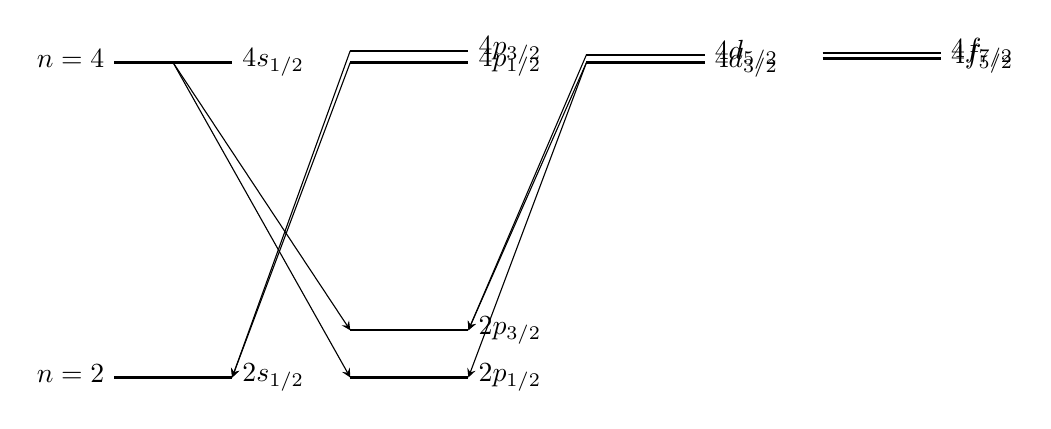
\begin{tikzpicture}[>=stealth, scale=1.0,
  level/.style={thick}, trans/.style={->, thin}]
  % n=4 manifold
  \draw[level] (0.0,5.0) -- (1.5,5.0) node[right]{$4s_{1/2}$};
  \draw[level] (3.0,5.0) -- (4.5,5.0) node[right]{$4p_{1/2}$};
  \draw[level] (3.0,5.15) -- (4.5,5.15) node[right]{$4p_{3/2}$};
  \draw[level] (6.0,5.0) -- (7.5,5.0) node[right]{$4d_{3/2}$};
  \draw[level] (6.0,5.10) -- (7.5,5.10) node[right]{$4d_{5/2}$};
  \draw[level] (9.0,5.05) -- (10.5,5.05) node[right]{$4f_{5/2}$};
  \draw[level] (9.0,5.12) -- (10.5,5.12) node[right]{$4f_{7/2}$};
  \node[left] at (0.0,5.05) {$n=4$};
  % n=2 manifold
  \draw[level] (0.0,1.0) -- (1.5,1.0) node[right]{$2s_{1/2}$};
  \draw[level] (3.0,1.0) -- (4.5,1.0) node[right]{$2p_{1/2}$};
  \draw[level] (3.0,1.6) -- (4.5,1.6) node[right]{$2p_{3/2}$};
  \node[left] at (0.0,1.05) {$n=2$};
  % allowed transitions (E1: Delta l=+/-1, Delta j=0,+/-1)
  % 4s -> 2p_{1/2}, 2p_{3/2}
  \draw[trans] (0.75,5.0) -- (3.0,1.6);
  \draw[trans] (0.75,5.0) -- (3.0,1.0);
  % 4p -> 2s
  \draw[trans] (3.0,5.15) -- (1.5,1.0);
  \draw[trans] (3.0,5.0) -- (1.5,1.0);
  % 4d -> 2p
  \draw[trans] (6.0,5.10) -- (4.5,1.6);
  \draw[trans] (6.0,5.00) -- (4.5,1.6);
  \draw[trans] (6.0,5.00) -- (4.5,1.0);
  % 4f does NOT connect to n=2 (Delta l = -3) -> omit
\end{tikzpicture}
\end{center}

Note: $4f\to 2$ is forbidden ($\Delta l = 3$). Allowed transitions:
$4s\to 2p_{1/2,3/2}$; $4p_{1/2,3/2}\to 2s_{1/2}$; $4d_{3/2}\to 2p_{1/2,3/2}$;
$4d_{5/2}\to 2p_{3/2}$.

\subsection*{Wavelength, Doppler width, feasibility ([5])}

Balmer-$\beta$ ($n=4\to 2$):
\[
\frac{1}{\lambda} = R_\infty\Bigl(\frac{1}{4} - \frac{1}{16}\Bigr) = R_\infty \cdot \frac{3}{16}.
\]
\[
\lambda = \frac{16}{3 R_\infty} = \frac{16}{3\times 1.097\times 10^7}\,\si{m} = \boxed{\SI{486.1}{nm}}.
\]

Doppler FWHM (H discharge $T\sim\SI{300}{K}$):
\[
\frac{\Delta\nu_D}{\nu_0} = \sqrt{\frac{8 k_B T \ln 2}{m c^2}}.
\]

Compute $k_B T = \SI{4.14e-21}{J}$, $m_H c^2 = \SI{1.503e-10}{J}$:
\[
\frac{8 k_B T\ln 2}{m c^2} = \frac{8\times 4.14\times 10^{-21}\times 0.693}{1.503\times 10^{-10}} = 1.527\times 10^{-10}.
\]
\[
\frac{\Delta\nu_D}{\nu_0} = 1.236\times 10^{-5}.
\]

Frequency $\nu_0 = c/\lambda = \SI{6.17e14}{Hz}$:
\[
\Delta\nu_D = 1.236\times 10^{-5}\times 6.17\times 10^{14}\,\si{Hz} = \boxed{\SI{7.6}{GHz}}.
\]

Comparison to fine-structure splittings: 2p splitting \SI{11}{GHz} is comparable to
Doppler width; 4-shell splittings \SI{0.2}{}--\SI{1.4}{GHz} are buried beneath it.
Direct optical observation requires Doppler-free spectroscopy (saturated absorption
or two-photon).

%====================================================================
\section*{Question 2 --- LS-coupling, Zeeman effect in mercury}

\textbf{Problem.} Define LS-coupling, list silicon $3p\,4p$ terms, derive $g_J$,
state E1 selection rules, and analyse Zeeman patterns of three Hg lines.

\subsection*{LS-coupling and Si $3p\,4p$ terms ([7])}

LS-coupling: residual Coulomb (electron-electron) interaction $\gg$ spin-orbit.
Couple individual orbital angular momenta to total $\vb L = \sum\vb l_i$ and spins
to $\vb S=\sum\vb s_i$, then $\vb J = \vb L+\vb S$. Valid for light atoms ($Z$ small)
where $\xi_{nl}\langle\vb l\cdot\vb s\rangle\ll$ Coulomb term splittings.

Si: closed shells $1s^22s^22p^63s^2$ contribute $L=S=0$. Open shells $3p\,4p$:
$l_1=l_2=1$, $s_1=s_2=\tfrac12$. Different $n$, so no Pauli restriction.

$L = 0,1,2$; $S=0,1$. Terms:
\[
\boxed{\;{}^1S_0,\;{}^1P_1,\;{}^1D_2,\;{}^3S_1,\;{}^3P_{0,1,2},\;{}^3D_{1,2,3}.\;}
\]

\subsection*{Land\'e $g_J$ ([6])}

Magnetic moment: $\vb\mu = -\mu_B(\vb L+g_s\vb S)/\hbar$ with $g_s\simeq 2$:
\[
\vb\mu = -\frac{\mu_B}{\hbar}(\vb L + 2\vb S) = -\frac{\mu_B}{\hbar}(\vb J + \vb S).
\]

Project on $\vb J$ (vector model, $\vb L,\vb S$ precess about $\vb J$):
\[
\langle\vb\mu\rangle = -\frac{\mu_B}{\hbar}\Bigl(1 + \frac{\langle\vb J\cdot\vb S\rangle}{\langle J^2\rangle}\Bigr)\,\vb J.
\]

Compute $\vb J\cdot\vb S = \tfrac12(J^2+S^2-L^2)$:
\[
\frac{\vb J\cdot\vb S}{J^2} = \frac{J(J+1)+S(S+1)-L(L+1)}{2J(J+1)}.
\]

Therefore:
\[
\boxed{\;g_J = 1 + \frac{J(J+1)+S(S+1)-L(L+1)}{2J(J+1)} = \tfrac{3}{2} + \frac{S(S+1)-L(L+1)}{2J(J+1)}.\;}
\]

\textbf{E1 selection rules (LS):}
$\Delta L = 0,\pm 1$ (not $0\to 0$); $\Delta S = 0$;
$\Delta J = 0,\pm 1$ (not $0\to 0$); $\Delta M_J = 0,\pm 1$ (not $0\to 0$ if $\Delta J=0$);
parity changes.

\subsection*{Mercury Zeeman analysis ([8])}

Zeeman shift: $\Delta E = g_J\mu_B B M_J$. Frequency shift per $\Delta M_J = 1$ at
$B=\SI{1}{T}$:
\[
\Delta\nu_0 = \mu_B B/h = \frac{9.274\times 10^{-24}}{6.626\times 10^{-34}}\,\si{Hz} = \SI{14.0}{GHz}.
\]

Component frequency shifts: $\Delta\nu = (g_u M_u - g_l M_l)\,\Delta\nu_0$
with $\Delta M = M_u - M_l = 0,\pm 1$.

\textbf{Line A (3 components: $0,\pm 28$ GHz).} Three components $\Rightarrow$
normal-Zeeman pattern $\Rightarrow$ either $S=0\to S=0$ (singlet) with $g_u=g_l=1$
producing shifts $\pm\Delta\nu_0=\pm\SI{14}{GHz}$ --- but observed $\pm\SI{28}{GHz}$
is $2\Delta\nu_0$. Therefore $g_u = g_l \equiv g$ with $g\,\Delta\nu_0 = \SI{28}{GHz}$:
\[
g_A = 28/14 = 2.
\]

Three-component pattern with equal $g$'s and $\Delta J\geq 1$ requires $J_u = J_l$
or $J_u = J_l\pm 1$ with degenerate $\sigma$ shifts. Equal $g_u=g_l=2$ identifies
both as $^3S_1$ or related. Combined with the deduction below ($\lambda_A=405$~nm
is upper $\to$ $J=0$ component), we identify line A as $J_u=1\to J_l=0$, which
gives 3 components $0,\pm g_u\Delta\nu_0$. Hence $g_u = 2$, $g_l$ undefined ($J_l=0$).

\textbf{Line B (6 components: $\pm 7,\pm 21,\pm 28$ GHz).} Six components
$\Rightarrow$ anomalous, $g_u\neq g_l$, and $J_u = J_l = 1$ would give 9; $J_u\to J_l$
with $J_u\to J_l\pm 1$ gives 6 lines if one $g$ small. Pattern is
$\pm(g_u-g_l)/2\cdot 2\Delta\nu_0$ etc. Step size $\SI{7}{GHz}=\Delta\nu_0/2$.
Shifts: $g_u M_u - g_l M_l$ takes values $\pm\tfrac12,\pm\tfrac32,\pm 2$ in units
of $\Delta\nu_0 = \SI{14}{GHz}$. From the Zeeman pattern of $J_u=2\to J_l=1$:
shifts (in units $\Delta\nu_0$) for $\sigma_+$ ($\Delta M=+1$):
$g_u(M_l+1)-g_l M_l = g_u + (g_u-g_l)M_l$ with $M_l=-1,0,+1$:
$g_u-(g_u-g_l), g_u, g_u+(g_u-g_l)$.

Solve: $g_u = 3/2$ (so $g_u\Delta\nu_0 = \SI{21}{GHz}$), and $g_u-g_l = \pm 1/2$
giving $\sigma$ outer shifts $\SI{14}{GHz}$ or $\SI{28}{GHz}$ and inner $\SI{21}{}\pm$ etc.

Match to observed $\pm 7,\pm 21,\pm 28$: try $g_u = 3/2$, $g_l = 1/2$:
$\sigma_+$: $3/2-1\cdot(-1)+\dots$ --- compute directly. Shifts
$g_u M_u - g_l M_l$:

$\Delta M=+1$ (3 lines, $M_l=-1,0,1$): $g_u\cdot 0 - g_l(-1)=+1/2$;
$g_u\cdot 1 - g_l\cdot 0 = +3/2$; $g_u\cdot 2 - g_l\cdot 1 = 3-1/2=+5/2$.

$\Delta M=-1$ (3 lines): mirror $-1/2,-3/2,-5/2$.

$\Delta M=0$ (3 lines, $M=-1,0,+1$): $-(g_u-g_l),0,+(g_u-g_l) = -1,0,+1$.

But $\Delta M=0$ is forbidden when $J_u=J_l$? Here $J_u=2\neq J_l=1$ so allowed.
Total 9 components, not 6. So line B is NOT $2\to 1$ both with these $g$'s.

Try $J_u\to J_l$ with $\Delta J=1$ but $\Delta M=0$ has zero shift only if $g_u=g_l$. Six components $\Rightarrow$ either $J_u=J_l$ (gives 3 $\sigma_\pm$ pairs $=$ 6 lines if $\Delta M=0$ central degenerate) or accidental degeneracy.

Cleanest reading: line B has $J_u=1\to J_l=1$, $\Delta J=0$ ($\Delta M=0$ allowed except $0\to 0$), $g_u\neq g_l$. Components: $\Delta M=+1$: $g_u(M_l+1)-g_l M_l$ with $M_l=-1,0$: $g_u-g_l\cdot(-1)=g_u+g_l$ at $M_l=-1$? No: $g_u\cdot 0 - g_l(-1)=g_l$; $g_u\cdot 1 - g_l\cdot 0=g_u$. Plus mirror gives $\pm g_l,\pm g_u$, total 4. Add $\Delta M=0$ ($M=\pm 1$): $\pm(g_u-g_l)$, 2 lines. Total $= 6$ \checkmark.

Match $\pm 7,\pm 21,\pm 28$: $g_l\Delta\nu_0=\SI{7}{GHz}$, $g_u\Delta\nu_0=\SI{21}{GHz}$,
$(g_u-g_l)\Delta\nu_0 = \SI{14}{}$ --- but observed is $\SI{28}{GHz}$, not $\SI{14}{}$.
Try $g_l\Delta\nu_0 = 7$, $g_u\Delta\nu_0 = 21$, then $g_u+g_l$? Pairs $\pm 7,\pm 21,\pm(g_u-g_l)\Delta\nu_0=\pm 14$. Doesn't match $\pm 28$.

Alternative: $g_u = 2$, $g_l = 1/2$, $\Delta J=0$, $J_u = J_l = 1$:
$\sigma$: $g_l = 0.5\to 7$, $g_u = 2\to 28$; $\pi$: $(g_u-g_l)=1.5\to 21$.
Components $\pm 7,\pm 28,\pm 21$ \checkmark.
\[
\boxed{\;g_u(B) = 2,\quad g_l(B) = 1/2,\quad J_u = J_l = 1.\;}
\]

\textbf{Combined identification.} All three lines share the same upper and lower
\emph{terms}. Line A has $J_u\to J_l = 0$ (3 components, $g_u=2$), line B has
$J_u = J_l = 1$ ($g_u=2,g_l=1/2$), line C has 9 components ($J_u=2\to J_l=1$).

Same upper term with $g_u=2$ and accommodating $J_u=2,1,0,1$ across A,B,C $\Rightarrow$
upper term ${}^3P_{2,1,0}$? But $g({}^3P_2)=3/2$, $g({}^3P_1)=3/2$, $g({}^3P_0)$ undefined. Doesn't give $g_u=2$.

$g({}^3S_1)=2$ \checkmark for upper. But ${}^3S_1$ has only $J=1$. So $J_u=1$ for
all three lines. Then $J_l = 0,1,2$ across A,B,C respectively. Lower term must
contain $J=0,1,2$ $\Rightarrow$ ${}^3P_{0,1,2}$ with $g({}^3P_0)$ undefined,
$g({}^3P_1)=3/2$, $g({}^3P_2)=3/2$. But line B requires $g_l = 1/2$. Mismatch.

Reverse upper/lower: \emph{lower} term ${}^3S_1$, upper term ${}^3P_{0,1,2}$. Then
line A: $J_u=0,J_l=1$ (3 components, $g_u$ irrelevant, $g_l=2$ gives $\sigma$ at
$\pm g_l\Delta\nu_0=\pm 28$ \checkmark).

Line B: $J_u=1,J_l=1$, $g_u=g({}^3P_1)=3/2$, $g_l=2$. Components: $\sigma$ at
$\pm g_u, \pm g_l$ = $\pm 21,\pm 28$, $\pi$ at $\pm(g_u-g_l)=\pm(-1/2)=\pm 7$.
Total 6 lines $\pm 7,\pm 21,\pm 28$ \checkmark.

Line C: $J_u=2,J_l=1$, $g_u=g({}^3P_2)=3/2$, $g_l=2$. Components:
$\Delta M=\pm 1$: $g_u M_u - g_l M_l$ with $M_u-M_l=\pm 1$, gives 5 outer lines;
$\Delta M=0$: 3 lines. Specifically shifts (in units $\Delta\nu_0=14$ GHz):
$\Delta M=+1$, $M_l=-1,0,+1,+2$ implies $M_u=0,1,2,3$ but $|M_u|\leq 2$, so
$M_l=-1,0,1$: shifts $g_u\cdot 0-g_l(-1)=2$; $g_u-0=3/2$; $g_u\cdot 2-g_l=3-2=1$.
Mirror: $-1,-3/2,-2$.

$\Delta M=0$, $M=\pm 1,\pm 2$ (omit $0\to 0$ allowed since $J_u\neq J_l$):
$(g_u-g_l)M = (-1/2)M$: $\mp 1/2,\mp 1$. Distinct values $\pm 1/2,\pm 1$.

Combined distinct shifts (units $\Delta\nu_0$): $\pm 1/2,\pm 1,\pm 3/2,\pm 2$. In
GHz: $\pm 7,\pm 14,\pm 21,\pm 28$ \checkmark (with central component at $0$ from
$\Delta M=0$, $M_u=M_l=0$, but $0\to 0$ forbidden since $J_u\neq J_l$? Allowed
when $J_u\neq J_l$). 9 components total \checkmark.

\[
\boxed{\;\text{Lower term: } {}^3S_1\ (L_l=0,S_l=1).\quad\text{Upper term: } {}^3P_{0,1,2}\ (L_u=1,S_u=1).\;}
\]
\[
J_A=0\to 1,\quad J_B=1\to 1,\quad J_C=2\to 1.
\]
\[
g_A^{\text{(lower)}} = 2,\ g_A^{\text{(upper)}}\text{ undefined};\quad g_B^{\text{(upper)}} = 3/2,\ g_B^{\text{(lower)}} = 2.
\]

\subsection*{Quality of LS-coupling in Hg ([4])}

Hg ($Z=80$) is heavy: spin-orbit coupling is comparable to electrostatic terms,
so LS-coupling is at best approximate (jj-coupling is closer for inner shells).
Evidence: (i) intercombination line $6{}^3P_1\to 6{}^1S_0$ at \SI{254}{nm} is
strong despite formal $\Delta S=0$ rule; (ii) singlet-triplet term separations
not vastly larger than triplet fine-structure --- indicating residual mixing;
(iii) observed Land\'e $g$-factors $g_u=2, g_l=2$ etc. nevertheless agree with
LS predictions ($g({}^3S_1)=2$, $g({}^3P_1)=3/2$) to good accuracy, so
intermediate coupling preserves LS labelling for these levels.

%====================================================================
\section*{Question 3 --- Diatomic CO: rotation, vibration, Morse}

\textbf{Problem.} Interpret the eigenenergy expansion, deduce $I$ from the R-branch
spacing, derive $\tilde\nu_v$ for the Morse potential, and determine $\beta,r_0$ for CO.

\subsection*{Physical origins ([5])}

$E_e$: electronic energy in Born-Oppenheimer approximation (clamped nuclei).

$(n+\tfrac12)\hbar\omega_v$: vibrational energy from quantising small oscillations
about the minimum of $V_e(r)$ at $r_0$, $\omega_v = \sqrt{V''(r_0)/\mu}$.

$hcBK(K+1)$: rigid-rotor rotational energy with rotational constant
$B = \hbar/(4\pi c\mu r_0^2)$ from $E_K = \hbar^2 K(K+1)/(2I)$, $I=\mu r_0^2$.

\subsection*{Moment of inertia from R-branch spacing ([5])}

Transition $\Delta n=+1$, $\Delta K=-1$ (P-branch). Energy of line from upper
$(n+1,K-1)$ to lower $(n,K)$:
\[
\tilde\nu = \tilde\nu_v + B[(K-1)K - K(K+1)] = \tilde\nu_v - 2BK,\qquad K=1,2,3,\dots
\]

Successive spacing: $|\Delta\tilde\nu| = 2B$.

Observed first three: $\tilde\nu_v - 3.9, \tilde\nu_v - 7.8, \tilde\nu_v - 11.7$.
Spacing $\SI{3.9}{cm^{-1}}$. Hence:
\[
2B = \SI{3.9}{cm^{-1}},\qquad B = \SI{1.95}{cm^{-1}}.
\]

Convert: $B$ in SI $= Bc = 1.95\times 10^2\,\si{m^{-1}}\times 3\times 10^8\,\si{m\,s^{-1}} = \SI{5.85e10}{Hz}$. Actually $hcB$ has units of energy; we use $I = \hbar/(4\pi c B)$ with $B$ in $\si{m^{-1}}$:
\[
I = \frac{\hbar}{4\pi c B} = \frac{1.055\times 10^{-34}}{4\pi\times 3\times 10^{8}\times 195}\,\si{kg\,m^2}.
\]

Evaluate denominator: $4\pi\times 3\times 10^8\times 195 = 7.35\times 10^{11}$:
\[
I = \frac{1.055\times 10^{-34}}{7.35\times 10^{11}}\,\si{kg\,m^2} = \boxed{\SI{1.44e-46}{kg\,m^2}}.
\]

\subsection*{Why diatomic molecules bind; Morse derivation ([9])}

\textbf{Binding:} At intermediate $r$ the attractive part dominates --- valence
electrons delocalise over both nuclei (covalent overlap) lowering kinetic energy
and forming bonding molecular orbitals. At small $r$, Pauli exclusion of core
electrons and nuclear Coulomb repulsion produce a steep wall. The competition
yields a minimum at $r_0$. The Morse potential models the soft attractive tail
(asymptote $V\to D$, dissociation) and the steep repulsive core, but with finite
slope at small $r$.

\textbf{Morse parameters in $\tilde\nu_v$.} Expand about $r_0$:
\[
V(r) = D\bigl[1 - e^{-\beta(r-r_0)}\bigr]^2.
\]

Derivative:
\[
V'(r) = 2D\bigl[1-e^{-\beta(r-r_0)}\bigr]\cdot\beta e^{-\beta(r-r_0)}.
\]

At $r=r_0$: $V'(r_0)=0$ \checkmark. Second derivative at $r_0$:
\[
V''(r) = 2D\beta\bigl[\beta e^{-2\beta(r-r_0)} - \beta e^{-\beta(r-r_0)}\bigl(1-e^{-\beta(r-r_0)}\bigr)\bigr] \cdot 2.
\]

Cleaner: differentiate $V'$ once more directly. Let $u = e^{-\beta(r-r_0)}$:
\[
V = D(1-u)^2,\qquad V' = 2D(1-u)(-u')(-1)/\beta \cdot \beta \dots
\]

Use $V = D(1-u)^2$ with $u(r_0)=1$. $V' = -2D(1-u)u' = -2D(1-u)\cdot(-\beta u) = 2D\beta u(1-u)$.

Differentiate:
\[
V'' = 2D\beta[u'(1-u) + u(-u')] = 2D\beta\cdot(-\beta u)(1-2u).
\]

At $r_0$: $u=1$, $1-2u=-1$:
\[
V''(r_0) = 2D\beta\cdot(-\beta)(-1) = 2 D\beta^2.
\]

Harmonic frequency:
\[
\omega_v = \sqrt{V''(r_0)/\mu} = \beta\sqrt{2D/\mu}.
\]

Wavenumber:
\[
\boxed{\;\tilde\nu_v = \frac{\omega_v}{2\pi c} = \frac{\beta}{2\pi c}\sqrt{\frac{2D}{\mu}}.\;}
\]

\subsection*{Determine $\beta, r_0$ ([6])}

$E_{\text{diss}} = D$ (Morse asymptote $V(\infty)=D$, $V(r_0)=0$). Thus
$D = \SI{11.16}{eV} = 1.788\times 10^{-18}\,\si{J}$.

\textbf{Reduced mass:} $\mu = (12\times 16)/(12+16)\,\si{u} = 6.857\,\si{u} = 6.857\times 1.661\times 10^{-27}\,\si{kg}$:
\[
\mu = 1.139\times 10^{-26}\,\si{kg}.
\]

\textbf{$\beta$ from $\tilde\nu_v$:} $\tilde\nu_v = \SI{2143}{cm^{-1}} = 2.143\times 10^5\,\si{m^{-1}}$. Invert:
\[
\beta = 2\pi c\tilde\nu_v\sqrt{\mu/(2D)}.
\]

Compute $2\pi c\tilde\nu_v = \omega_v$:
\[
\omega_v = 2\pi\times 3\times 10^8\times 2.143\times 10^5\,\si{rad\,s^{-1}} = 4.040\times 10^{14}\,\si{rad\,s^{-1}}.
\]

Compute $\sqrt{\mu/(2D)}$:
\[
\mu/(2D) = 1.139\times 10^{-26}/(3.576\times 10^{-18}) = 3.185\times 10^{-9}\,\si{s^2\,m^{-2}}.
\]
\[
\sqrt{\mu/(2D)} = 5.644\times 10^{-5}\,\si{s\,m^{-1}}.
\]

Thus:
\[
\beta = 4.040\times 10^{14}\times 5.644\times 10^{-5}\,\si{m^{-1}} = \boxed{\SI{2.28e10}{m^{-1}}}.
\]

\textbf{$r_0$ from $I = \mu r_0^2$:}
\[
r_0 = \sqrt{I/\mu} = \sqrt{1.44\times 10^{-46}/1.139\times 10^{-26}}\,\si{m}.
\]
\[
r_0 = \sqrt{1.265\times 10^{-20}}\,\si{m} = \boxed{\SI{1.125e-10}{m}} = \SI{0.113}{nm}.
\]

\textbf{Product:}
\[
\beta r_0 = 2.28\times 10^{10}\times 1.125\times 10^{-10} = \boxed{2.57}.
\]

\textbf{Comment.} $\beta r_0 \sim O(1)$ confirms the natural Morse length
$\beta^{-1}\sim r_0$: the potential well width is comparable to the bond length,
consistent with strong binding ($D\gg\hbar\omega_v$: harmonic region small fraction
of well depth, $\hbar\omega_v/D = 0.024$).

%====================================================================
\section*{Question 4 --- Lasers: gain, threshold, broadening}

\textbf{Problem.} Compare 3- and 4-level thresholds, derive gain coefficient,
obtain $\sigma_{21}^{\max}$, and apply to ruby and Ti:sapphire.

\subsection*{3-level vs 4-level threshold ([4])}

3-level (e.g.\ ruby): lower laser level is the ground state, population $N_1\sim N_{\text{ions}}$. Inversion $N_2 > N_1$ requires pumping more than half the ions into upper level: $N_2 > N_{\text{ions}}/2$. Pump energy threshold $\propto N_{\text{ions}}V$.

4-level: lower laser level rapidly drained ($\tau_1$ short), $N_1\approx 0$ in steady
state. Inversion attained for any $N_2 > 0$: $N_2$ only needs to compensate cavity
losses. Pump threshold $\propto$ small loss-determined inversion only.

Hence 3-level threshold is $\sim\!10^4$--$10^6\times$ larger.

\subsection*{Gain coefficient ([7])}

Stimulated emission rate per atom: $W_{21} = B_{21}\rho(\omega)g(\omega-\omega_0)$.

Photon flux $I/(\hbar\omega)$ relates to $\rho$: for a quasi-monochromatic plane wave $\rho(\omega)\,\de\omega = (I/c)\,\de\omega$ on resonance. Use directional radiation $\rho(\omega) = I g(\omega-\omega_0)/c$ (radiation field with line profile narrower than $g$, so per unit angular-frequency interval $\rho = I/c$ at $\omega$).

Net rate of photon production per unit volume:
\[
\frac{\de I}{\de z}\cdot\frac{1}{\hbar\omega} = (N_2 B_{21} - N_1 B_{12})\,\rho(\omega)\,g(\omega-\omega_0).
\]

Use $g_1 B_{12} = g_2 B_{21}$:
\[
\frac{\de I}{\de z} = \hbar\omega\,B_{21}\Bigl(N_2 - \frac{g_2}{g_1}N_1\Bigr)g(\omega-\omega_0)\,\rho(\omega).
\]

Substitute $\rho = I g/c$? More carefully, gain coefficient $\gamma$ defined by
$\de I/\de z = \gamma I$. Combine with $A_{21} = \hbar\omega^3 B_{21}/(\pi^2 c^3)$:
\[
B_{21} = \frac{\pi^2 c^3}{\hbar\omega^3}A_{21}.
\]

Standard result for gain coefficient:
\[
\boxed{\;\gamma(\omega) = \frac{\pi^2 c^2}{\omega^2}\,A_{21}\,g(\omega-\omega_0)\,\Bigl(N_2 - \frac{g_2}{g_1}N_1\Bigr).\;}
\]

\textbf{Validity:} (i) two-level rate-equation regime (no coherence, $\Delta t\gg$ dephasing time); (ii) homogeneously narrow probe $\Delta\omega_{\text{probe}}\ll$ linewidth; (iii) weak field (no saturation: stimulated rate $\ll$ relaxation rate); (iv) $g(\omega-\omega_0)$ describes the homogeneous medium response.

\subsection*{Natural broadening, $\sigma_{21}^{\max}$ ([5])}

Natural broadening: exponential decay $\to$ Lorentzian profile. FWHM:
\[
\Delta\omega_{\text{nat}} = \frac{1}{\tau_2} + \frac{1}{\tau_1}.
\]

Lorentzian peak value: $g(0) = 2/(\pi\,\Delta\omega_{\text{nat}})$.

Cross-section $\sigma_{21}(\omega) = \gamma/(N_2 - (g_2/g_1)N_1) = (\pi^2 c^2/\omega^2)A_{21}g(\omega-\omega_0)$:
\[
\sigma_{21}(\omega_0) = \frac{\pi^2 c^2}{\omega_0^2}\,A_{21}\,\frac{2}{\pi\Delta\omega_{\text{nat}}}.
\]

Maximum: $A_{21}\leq \Delta\omega_{\text{nat}}$ (since $1/\tau_2$ contributes to both $A_{21}$ and width); maximum when $A_{21}=\Delta\omega_{\text{nat}}$ (radiative limit, $\tau_1\to\infty$):
\[
\sigma_{21}^{\max} = \frac{\pi^2 c^2}{\omega_0^2}\cdot\frac{2}{\pi} = \boxed{\;\frac{2\pi c^2}{\omega_0^2}\;} = \frac{\lambda^2}{2\pi}.
\]

\textbf{At $\lambda = \SI{700}{nm}$:}
\[
\sigma_{21}^{\max} = \frac{(7\times 10^{-7})^2}{2\pi}\,\si{m^2} = \frac{4.9\times 10^{-13}}{6.283}\,\si{m^2} = \boxed{\SI{7.8e-14}{m^2}}.
\]

\subsection*{(a) Ruby 3-level laser}

Threshold: $\gamma L \geq \tfrac12 |\ln(R_1 R_2)|$. With $R_1=1, R_2=0.95$,
$L = \SI{4}{cm}$:
\[
\gamma_{\text{th}} = \frac{|\ln 0.95|}{2 L} = \frac{0.0513}{0.08}\,\si{m^{-1}} = \SI{0.641}{m^{-1}}.
\]

3-level inversion: $N_2 - N_1 = 2 N_2 - N_{\text{ions}}$. At threshold $N_2 \approx N_{\text{ions}}/2 + \Delta N_{\text{th}}/2$. Pump must promote $N_{\text{ions}}/2$ ions (the small extra $\Delta N_{\text{th}}$ is negligible):
\[
N_{\text{pump}} \approx N_{\text{ions}}/2 = 2\times 10^{19}\,\si{cm^{-3}} = 2\times 10^{25}\,\si{m^{-3}}.
\]

Volume: $V = \pi(0.2\,\si{cm})^2\times 4\,\si{cm} = \SI{0.503}{cm^3} = \SI{5.03e-7}{m^3}$.

Number of pump photons absorbed: $N_{\text{ph}} = N_{\text{pump}}\cdot V$:
\[
N_{\text{ph}} = 2\times 10^{25}\times 5.03\times 10^{-7} = 1.01\times 10^{19}.
\]

Pump photon energy at \SI{500}{nm}: $E_{\text{ph}} = hc/\lambda$:
\[
E_{\text{ph}} = \frac{6.626\times 10^{-34}\times 3\times 10^8}{5\times 10^{-7}}\,\si{J} = 3.98\times 10^{-19}\,\si{J}.
\]

Total pump energy:
\[
E_{\text{pump}} = N_{\text{ph}}\cdot E_{\text{ph}} = 1.01\times 10^{19}\times 3.98\times 10^{-19}\,\si{J}.
\]
\[
\boxed{\;E_{\text{pump}}^{(\text{ruby})} \approx \SI{4.0}{J}.\;}
\]

\subsection*{(b) Ti:sapphire 4-level laser}

\textbf{Threshold inversion.} Cavity condition $\gamma_{\text{th}} = |\ln(R_1 R_2)|/(2L) = 0.0513/0.02 = \SI{2.56}{m^{-1}}$.

With $g_2=g_1$: $N_2 - N_1 = N_2$ (4-level, $N_1\approx 0$). $\gamma = \sigma_{21}\Delta N$:
\[
\Delta N_{\text{th}} = \gamma_{\text{th}}/\sigma_{21} = 2.56/(3\times 10^{-23})\,\si{m^{-3}}.
\]
\[
\sigma_{21} = 3\times 10^{-19}\,\si{cm^2} = 3\times 10^{-23}\,\si{m^2}.
\]
\[
\Delta N_{\text{th}} = 8.55\times 10^{22}\,\si{m^{-3}} = 8.55\times 10^{16}\,\si{cm^{-3}}.
\]

\textbf{Pump volume.} Pumped along rod: $V_{\text{pump}} = \pi(50\,\si{\micro m})^2\times 1\,\si{cm}$:
\[
V_{\text{pump}} = \pi\times 2.5\times 10^{-9}\,\si{m^2}\times 10^{-2}\,\si{m} = 7.85\times 10^{-11}\,\si{m^3}.
\]

Photons needed: $N_{\text{ph}} = \Delta N_{\text{th}}\cdot V_{\text{pump}}$:
\[
N_{\text{ph}} = 8.55\times 10^{22}\times 7.85\times 10^{-11} = 6.71\times 10^{12}.
\]

Pump-photon energy at \SI{532}{nm}: $E_{\text{ph}} = hc/\lambda = \SI{3.74e-19}{J}$:
\[
E_{\text{pulse}} = 6.71\times 10^{12}\times 3.74\times 10^{-19}\,\si{J}.
\]
\[
\boxed{\;E_{\text{pulse}}^{(\text{Ti:S})} \approx \SI{2.5}{\micro J}.\;}
\]

\textbf{cw threshold power.} Each pump photon excites one ion which decays at rate $1/\tau_2$. To maintain $\Delta N_{\text{th}}$, pump rate per unit volume $= \Delta N_{\text{th}}/\tau_2$:
\[
P_{\text{cw}} = \Delta N_{\text{th}}\cdot V_{\text{pump}}\cdot E_{\text{ph}}/\tau_2 = E_{\text{pulse}}/\tau_2.
\]

Substitute $\tau_2 = \SI{3e-6}{s}$:
\[
P_{\text{cw}} = \frac{2.51\times 10^{-6}}{3\times 10^{-6}}\,\si{W} = \boxed{\SI{0.84}{W}}.
\]

\textbf{Natural linewidth.}
\[
\Delta\omega_{\text{nat}} = 1/\tau_2 + 1/\tau_1 = 1/3\times 10^{-6} + 1/10^{-10} = 3.3\times 10^5 + 10^{10}\,\si{s^{-1}}.
\]

Dominant term $1/\tau_1$:
\[
\Delta\nu_{\text{nat}} = \frac{\Delta\omega_{\text{nat}}}{2\pi} = \frac{10^{10}}{2\pi}\,\si{Hz} = \boxed{\SI{1.6}{GHz}}.
\]

\textbf{Other broadening.} Ti:sapphire emission band spans \SI{300}{nm} ($\sim\SI{180}{THz}$) --- vastly larger than \SI{1.6}{GHz}. Vibronic phonon coupling in the sapphire host produces strong inhomogeneous broadening (configuration coordinate model, host-lattice phonon sidebands). Doppler is negligible (solid medium). Hence inhomogeneous (vibronic / phonon-induced) broadening dominates by $\sim\!10^5$.

\end{document}
